\documentclass{article}
\usepackage{amsmath,amssymb,listings,upquote}
\usepackage[margin=3cm]{geometry}
\usepackage{graphicx,color}
\lstset{language=Python}
\usepackage{enumerate}


\newcounter{zone}
\setcounter{zone}{0}
\newcommand{\zone}{\clearpage\refstepcounter{zone}\section*{Zone \arabic{zone}}}
\newcounter{question}
\setcounter{question}{0}
\newcounter{variant}
\newcounter{questionpoints}
\newcommand{\question}[1]{\newpage \refstepcounter{question} \setcounter{variant}{0} \setcounter{questionpoints}{#1}}
\newcommand{\variant}{\vspace{4em}\refstepcounter{variant}\noindent \arabic{question}/\arabic{variant}. (\arabic{questionpoints} point\ifnum \thequestionpoints > 1 s\fi) }
\newenvironment{answers}{\begin{enumerate}}{\end{enumerate}}
\newcommand{\answer}{\item }
\newcommand{\correctanswer}{\item $\bigstar$ }
\renewcommand{\theenumi}{\Alph{enumi}}
\newenvironment{solution}{{\bf Solution.} }{\vspace*{.3in}\hrule}



\begin{document}
	
	\newcount\maxrawpages
	\newcount\maxpadpages
	\newcount\minpadpages
	\maxrawpages=0
	\maxpadpages=0
	\minpadpages=1000000
	\newcount\padcount
	
	%%%%%%%%%%%%%%%%%%%%%%%%%%%%%%%%%%%%%%%%%%%%%%%%%%%%%%%%%%%%%%%%%%%%%%
	%%%%%%%%%%%%%%%%%%%%%%%%%%%%%%%%%%%%%%%%%%%%%%%%%%%%%%%%%%%%%%%%%%%%%%
	%%%%%%%%%%%%%%%%%%%%%%%%%%%%%%%%%%%%%%%%%%%%%%%%%%%%%%%%%%%%%%%%%%%%%%
	%%%%%%%%%%%%%%%%%%%%%%%%%%%%%%%%%%%%%%%%%%%%%%%%%%%%%%%%%%%%%%%%%%%%%%
	\cleardoublepage
	% Exam number 1
	
	\message{Exam 1/50}
	\setcounter{page}{1}
	
	
	\begin{center}
		%\textbf{\Large CS 101 Midterm \#1}
		%
		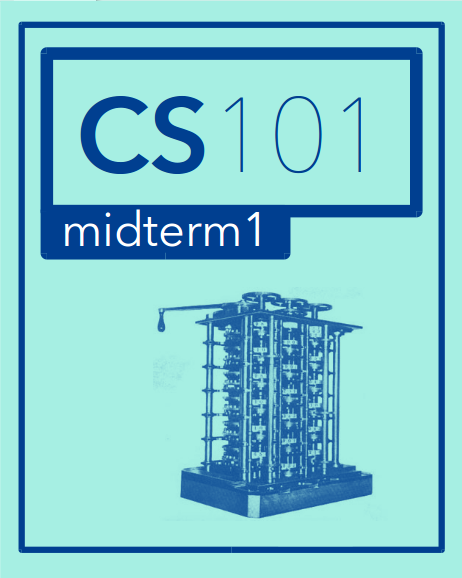
\includegraphics[width=2in]{../img/midterm1-header.png}
	\end{center}
	
	\bigskip
	\noindent
	\begin{itemize}
		\item \textbf{Be sure to enter your \underline{student ID} and \underline{your answers to questions} on your answer sheet}.
		\item Do not turn this page until instructed to do so.
		\item There are 30 questions, worth 1 point each.
		\item Each question has only \textbf{one} correct answer.
		\item You must not communicate with other students during this test.
		\item No books, notes, or electronic devices are permitted. In other words, you are not allowed to use a dictionary on your mobile phone or other electronic devices. However, if you don't understand the meaning of a particular English word in this exam, please raise your hand and the instructor will explain the meaning of the English word to you. 
		\item This is a 120-minute exam but you can finish the exam earlier than this 120-minute period.
		%\item There are several different versions of this exam.
	\end{itemize}


\newpage

% Zone 1


%%%%%%%%%%%%%%%%%%%%%%%%%%%%%%%%%%%%%%%%%%%%%%%%%%%%%%%%%



\newpage
\noindent
1. (1 point)
Consider the following program:
\begin{verbatim}
s="ECTOR"
t="GAWAIN"
x=len(str(s.isupper()))-t.find("A")
\end{verbatim}
What is the \textbf{type} of \texttt{x} after this program is executed?


\begin{enumerate}
\item[(A)]
\begin{verbatim}Boolean\end{verbatim}

\item[(B)]
\begin{verbatim}String\end{verbatim}

\item[(C)] $\bigstar$ 
\begin{verbatim}Integer\end{verbatim}

\item[(D)]
\begin{verbatim}None\end{verbatim}

\item[(E)]
\begin{verbatim}Float\end{verbatim}

\end{enumerate}

\vspace*{2em}
\hrule
\vspace{2em}

\noindent {\bf Solution.} 
\vspace{2em}
\hrule height 2pt


\newpage
\noindent
2. (1 point)
Consider the following incomplete program.
\begin{verbatim}
sum=0
for i in range(0,100):
    ???

\end{verbatim}
The program is intended to sum all of the integers between 1 and 100 (inclusive). What should replace the three question marks to complete the program?


\begin{enumerate}
\item[(A)]
\begin{verbatim}sum=sum+1\end{verbatim}

\item[(B)] $\bigstar$ 
\begin{verbatim}sum=sum+i+1 \end{verbatim}

\item[(C)]
\begin{verbatim}sum+1=sum \end{verbatim}

\item[(D)]
\begin{verbatim}sum=sum+i \end{verbatim}

\end{enumerate}

\vspace*{2em}
\hrule
\vspace{2em}

\noindent {\bf Solution.} 
\vspace{2em}
\hrule height 2pt


\newpage
\noindent
3. (1 point)
For this problem, you should compose a function which accomplishes a given task using the available code blocks arranged in the correct functional order.  \emph{We ignore indentation for this problem.}

\texttt{find\_max} should accept a \texttt{list} and return the value of the maximum item in the \texttt{list}.  (\texttt{None} is always the lowest value in any numeric comparison, so you may use it as an initializer.)

\begin{verbatim}
def find_max(my_list):
\end{verbatim}

\begin{enumerate}[1]
\item \texttt{max\_val = i}
\item \texttt{max\_val = None}
\item \texttt{for i in range(len(my\_list)):}
\item \texttt{if i > max\_val:}
\item \texttt{max\_val = my\_list[i]}
\item \texttt{return max\_val}
\item \texttt{for i in range(my\_list):}
\item \texttt{if my\_list[i] > max\_val:}
\item \texttt{print(max\_val)}
\end{enumerate}



\begin{enumerate}
\item[(A)]
2, 3, 8, 1, 6

\item[(B)]
2, 7, 4, 5, 6

\item[(C)]
2, 3, 4, 1, 6

\item[(D)] $\bigstar$ 
2, 3, 8, 5, 6

\item[(E)]
3, 2, 8, 5, 9

\end{enumerate}

\vspace*{2em}
\hrule
\vspace{2em}

\noindent {\bf Solution.} 
\vspace{2em}
\hrule height 2pt


\newpage
\noindent
4. (1 point)
How can the following mathematical equation be implemented as a Python expression? Assume \verb|a|, \verb|b|, and \verb|sin| have already been defined.
$$a \sin(a^b - b)$$


\begin{enumerate}
\item[(A)]
None of the other answers are correct.

\item[(B)]
\begin{verbatim}a*sin(a^b - b)\end{verbatim}

\item[(C)]
\begin{verbatim}a sin(a**b - b)\end{verbatim}

\item[(D)] $\bigstar$ 
\begin{verbatim}a*sin(a**b - b)\end{verbatim}

\item[(E)]
\begin{verbatim}a*sin(b^a - b)\end{verbatim}

\end{enumerate}

\vspace*{2em}
\hrule
\vspace{2em}

\noindent {\bf Solution.} 
\vspace{2em}
\hrule height 2pt


\newpage
\noindent
5. (1 point)
Consider the following program:
\begin{verbatim}
x=3
a=5
if (a%3)==2:
    x=x**3
elif(a%3)==1:
    x=x**2
else:
    x=x**1
\end{verbatim}
What is the \textbf{value} of \texttt{x} after this program is executed?


\begin{enumerate}
\item[(A)]
\begin{verbatim}9\end{verbatim}

\item[(B)] $\bigstar$ 
\begin{verbatim}27\end{verbatim}

\item[(C)]
None of the other answers are correct.

\item[(D)]
\begin{verbatim}3\end{verbatim}

\item[(E)]
\begin{verbatim}1\end{verbatim}

\end{enumerate}

\vspace*{2em}
\hrule
\vspace{2em}

\noindent {\bf Solution.} 
\vspace{2em}
\hrule height 2pt


\newpage
\noindent
6. (1 point)
Consider the following program:
\begin{verbatim}
x=0
for i in range(4,10):
    if i%3==0:
        x+=3
    elif i%2==0:
        x+=2
    else:
        x+=1
\end{verbatim}
What is the \textbf{value} of \texttt{x} after this program is executed?


\begin{enumerate}
\item[(A)]
\begin{verbatim}10\end{verbatim}

\item[(B)] $\bigstar$ 
\begin{verbatim}12\end{verbatim}

\item[(C)]
\begin{verbatim}11\end{verbatim}

\item[(D)]
\begin{verbatim}14\end{verbatim}

\item[(E)]
\begin{verbatim}13\end{verbatim}

\end{enumerate}

\vspace*{2em}
\hrule
\vspace{2em}

\noindent {\bf Solution.} 
\vspace{2em}
\hrule height 2pt


\newpage
\noindent
7. (1 point)
Evaluate the following expression:
\begin{verbatim}
[1,2]+[len("3")]
\end{verbatim}
What value is produced?


\begin{enumerate}
\item[(A)] $\bigstar$ 
\begin{verbatim}[1,2,1]\end{verbatim}

\item[(B)]
\begin{verbatim}[1,2,"3"]\end{verbatim}

\item[(C)]
\begin{verbatim}[1,2,1,2,1,2]\end{verbatim}

\item[(D)]
\begin{verbatim}[1,2,3]\end{verbatim}

\end{enumerate}

\vspace*{2em}
\hrule
\vspace{2em}

\noindent {\bf Solution.} 
\vspace{2em}
\hrule height 2pt


\newpage
\noindent
8. (1 point)
Consider the following program.
\begin{verbatim}
kay = 2
wart = 3

def knight(kay,wart):
    wart += 2
    kay += 3
    return wart + kay

wart = knight(kay, kay) + knight(wart, wart)
\end{verbatim}
After it is run, what is the final \textbf{value} of \texttt{wart}?


\begin{enumerate}
\item[(A)]
\begin{verbatim}5\end{verbatim}

\item[(B)] $\bigstar$ 
None of the other answers are correct.

\item[(C)]
\begin{verbatim}2\end{verbatim}

\item[(D)]
\begin{verbatim}3\end{verbatim}

\end{enumerate}

\vspace*{2em}
\hrule
\vspace{2em}

\noindent {\bf Solution.} 
\vspace{2em}
\hrule height 2pt


\newpage
\noindent
9. (1 point)
Consider the following program:
\begin{verbatim}
a=3
b=4
if a==3:
    b=a
elif a==4:
    a=5
else:
    a=b
\end{verbatim}
What is the \textbf{value} of a after this program is executed?


\begin{enumerate}
\item[(A)]
\begin{verbatim}7\end{verbatim}

\item[(B)]
None of the other answers are correct.

\item[(C)]
\begin{verbatim}4\end{verbatim}

\item[(D)] $\bigstar$ 
\begin{verbatim}3\end{verbatim}

\item[(E)]
\begin{verbatim}5\end{verbatim}

\end{enumerate}

\vspace*{2em}
\hrule
\vspace{2em}

\noindent {\bf Solution.} 
\vspace{2em}
\hrule height 2pt


\newpage
\noindent
10. (1 point)
Consider the following program.
\begin{verbatim}
s="ABCBA"
x=0
y=len(s)-1
while s[x]==s[y] and x<=y:
    x+=1
    y-=1
\end{verbatim}
After it is run, what is the final \textbf{value} of \texttt{x}?


\begin{enumerate}
\item[(A)] $\bigstar$ 
\begin{verbatim}3\end{verbatim}

\item[(B)]
\begin{verbatim}0\end{verbatim}

\item[(C)]
\begin{verbatim}1\end{verbatim}

\item[(D)]
\begin{verbatim}4\end{verbatim}

\item[(E)]
\begin{verbatim}2\end{verbatim}

\end{enumerate}

\vspace*{2em}
\hrule
\vspace{2em}

\noindent {\bf Solution.} 
\vspace{2em}
\hrule height 2pt


\newpage
\noindent
11. (1 point)
Consider the following program:
\begin{verbatim}
pi="3.14159"
e="2.71828"
x=pi*len(e)+pi
\end{verbatim}
What is the \textbf{type} of \texttt{x} after this program is executed?


\begin{enumerate}
\item[(A)]
\begin{verbatim}None\end{verbatim}

\item[(B)] $\bigstar$ 
\begin{verbatim}String\end{verbatim}

\item[(C)]
\begin{verbatim}Integer\end{verbatim}

\item[(D)]
\begin{verbatim}Boolean\end{verbatim}

\item[(E)]
\begin{verbatim}Float\end{verbatim}

\end{enumerate}

\vspace*{2em}
\hrule
\vspace{2em}

\noindent {\bf Solution.} 
\vspace{2em}
\hrule height 2pt


\newpage
\noindent
12. (1 point)
Consider the following program:
\begin{verbatim}
x="KING ARTHUR-MORGANA LEFAY-SIR BEDIVERE".split("-")
y=x[:]
y.reverse()
\end{verbatim}
What is the \textbf{value} of \texttt{x} after this program is executed?


\begin{enumerate}
\item[(A)]
\begin{verbatim}['KING', 'ARTHUR-MORGANA', 'LEFAY-SIR', 'BEDIVERE']\end{verbatim}

\item[(B)]
\begin{verbatim}['SIR BEDIVERE', 'MORGANA LEFAY', 'KING ARTHUR']\end{verbatim}

\item[(C)] $\bigstar$ 
\begin{verbatim}['KING ARTHUR', 'MORGANA LEFAY', 'SIR BEDIVERE']\end{verbatim}

\item[(D)]
\begin{verbatim}None\end{verbatim}

\item[(E)]
\begin{verbatim}['BEDIVERE', 'LEFAY-SIR', 'ARTHUR-MORGANA', 'KING']\end{verbatim}

\end{enumerate}

\vspace*{2em}
\hrule
\vspace{2em}

\noindent {\bf Solution.} 
\vspace{2em}
\hrule height 2pt


\newpage
\noindent
13. (1 point)
What is the result of the following expression?
\begin{verbatim}
[ 1, 2, 3 ] * 3.0
\end{verbatim}


\begin{enumerate}
\item[(A)]
\begin{verbatim}[1.0, 2.0, 3.0, 1.0, 2.0, 3.0, 1.0, 2.0, 3.0]\end{verbatim}

\item[(B)] $\bigstar$ 
\begin{verbatim}[1, 2, 3, 1, 2, 3, 1, 2, 3]\end{verbatim}

\item[(C)]
\begin{verbatim}None of the above.\end{verbatim}

\item[(D)]
\begin{verbatim}[3.0, 6.0, 9.0]\end{verbatim}

\item[(E)]
\begin{verbatim}[3, 6, 9]\end{verbatim}

\end{enumerate}

\vspace*{2em}
\hrule
\vspace{2em}

\noindent {\bf Solution.} 
\vspace{2em}
\hrule height 2pt


\newpage
\noindent
14. (1 point)
Consider the following program:
\begin{verbatim}
s="-B-O-R-S-"
x=s.split("-")[2:-2]
\end{verbatim}
What is the \textbf{value} of \texttt{x} after this program is executed?


\begin{enumerate}
\item[(A)]
\begin{verbatim}'ORS'\end{verbatim}

\item[(B)]
\begin{verbatim}''\end{verbatim}

\item[(C)]
\begin{verbatim}False\end{verbatim}

\item[(D)]
\begin{verbatim}None\end{verbatim}

\item[(E)] $\bigstar$ 
\begin{verbatim}['O', 'R']\end{verbatim}

\end{enumerate}

\vspace*{2em}
\hrule
\vspace{2em}

\noindent {\bf Solution.} 
\vspace{2em}
\hrule height 2pt


\newpage
\noindent
15. (1 point)
Consider the following program.
\begin{verbatim}
def artificing(s):
    return s+"%i" % 2
    return s*2
    return s

s=artificing("MERLIN")
\end{verbatim}
After it is run, what is the final \textbf{value} of s?


\begin{enumerate}
\item[(A)]
\begin{verbatim}None\end{verbatim}

\item[(B)]
\begin{verbatim}0\end{verbatim}

\item[(C)]
\begin{verbatim}"MERLINMERLIN"\end{verbatim}

\item[(D)] $\bigstar$ 
\begin{verbatim}"MERLIN2"\end{verbatim}

\item[(E)]
\begin{verbatim}"MERLIN%i"\end{verbatim}

\end{enumerate}

\vspace*{2em}
\hrule
\vspace{2em}

\noindent {\bf Solution.} 
\vspace{2em}
\hrule height 2pt


\newpage
\noindent
16. (1 point)
Consider the following program.
\begin{verbatim}
x=[]
for j in range(0,5):
    if (j%4)==0:
        x.append("-")
    if (j%5)==0:
        x.append("*")
\end{verbatim}
After it is run, what is the final \textbf{value} of \texttt{x}?


\begin{enumerate}
\item[(A)] $\bigstar$ 
\begin{verbatim}["-","*","-"]\end{verbatim}

\item[(B)]
None of the other answers are correct.

\item[(C)]
\begin{verbatim}["-","-","*"]\end{verbatim}

\item[(D)]
\begin{verbatim}["-","*"]\end{verbatim}

\item[(E)]
\begin{verbatim}["-","*","*"]\end{verbatim}

\end{enumerate}

\vspace*{2em}
\hrule
\vspace{2em}

\noindent {\bf Solution.} 
\vspace{2em}
\hrule height 2pt


\newpage
\noindent
17. (1 point)
Consider the following program:
\begin{verbatim}
a=["merlin","sir agravaine","king pellinore"]
b=[ ]
for i in range(0,3):
    b.append(a[0-i].title())
\end{verbatim}
What is the \textbf{value} of b after this program is executed?


\begin{enumerate}
\item[(A)]
\begin{verbatim}[ ]\end{verbatim}

\item[(B)]
\begin{verbatim}['Sir Agravaine', 'King Pellinore']\end{verbatim}

\item[(C)]
\begin{verbatim}['King Pellinore', 'Sir Agravaine']\end{verbatim}

\item[(D)]
\begin{verbatim}['King Pellinore', 'Sir Agravaine', 'Merlin']\end{verbatim}

\item[(E)] $\bigstar$ 
\begin{verbatim}['Merlin', 'King Pellinore', 'Sir Agravaine']\end{verbatim}

\end{enumerate}

\vspace*{2em}
\hrule
\vspace{2em}

\noindent {\bf Solution.} 
\vspace{2em}
\hrule height 2pt


\newpage
\noindent
18. (1 point)
Consider the following program:
\begin{verbatim}
x=[1,2,3]
def f(a):
    s=""
    a.append(4)
    for i in a:
        s+=str(i)
    return s

x.append(f(x))
\end{verbatim}
What is the \textbf{value} of \texttt{x} after this program is executed?


\begin{enumerate}
\item[(A)] $\bigstar$ 
\begin{verbatim}[1, 2, 3, 4, '1234']\end{verbatim}

\item[(B)]
\begin{verbatim}[1, 2, 3, '123']\end{verbatim}

\item[(C)]
\begin{verbatim}[1, 2, 3, 10]\end{verbatim}

\item[(D)]
\begin{verbatim}[1, 2, 3]\end{verbatim}

\item[(E)]
\begin{verbatim}[1, 2, 3, '1234']\end{verbatim}

\end{enumerate}

\vspace*{2em}
\hrule
\vspace{2em}

\noindent {\bf Solution.} 
\vspace{2em}
\hrule height 2pt


\newpage
\noindent
19. (1 point)
Consider the following program:
\begin{verbatim}
a=["S","T","U","P","E","F","Y"]
a=a[0:4]
a.sort()
x=""
for e in a:
    x=e+x
\end{verbatim}
What is the \textbf{value} of \texttt{x} after this program is executed?


\begin{enumerate}
\item[(A)]
None of the other answers are correct.

\item[(B)] $\bigstar$ 
\begin{verbatim}"UTSP"\end{verbatim}

\item[(C)]
\begin{verbatim}"PSTU"\end{verbatim}

\item[(D)]
\begin{verbatim}"STUP"\end{verbatim}

\item[(E)]
\begin{verbatim}"PUST"\end{verbatim}

\end{enumerate}

\vspace*{2em}
\hrule
\vspace{2em}

\noindent {\bf Solution.} 
\vspace{2em}
\hrule height 2pt


\newpage
\noindent
20. (1 point)
Consider the following incomplete Python program.
\begin{verbatim}
s="".join(["2","2","0","1"])
x=0
for i in range(len(s)-1):
    x+=int(???)
\end{verbatim}
What should replace the three question marks so the resulting value of \texttt{x} is 43?


\begin{enumerate}
\item[(A)]
\begin{verbatim}s[i:i-1]\end{verbatim}

\item[(B)]
\begin{verbatim}s[i+1:i+2]\end{verbatim}

\item[(C)]
\begin{verbatim}s[i:i+1]\end{verbatim}

\item[(D)] $\bigstar$ 
\begin{verbatim}s[i:i+2]\end{verbatim}

\end{enumerate}

\vspace*{2em}
\hrule
\vspace{2em}

\noindent {\bf Solution.} 
\vspace{2em}
\hrule height 2pt


\newpage
\noindent
21. (1 point)
\begin{verbatim}
x=str(3)+"str(3)"
\end{verbatim}
What is the \textbf{value} of \texttt{x} after this program is executed?


\begin{enumerate}
\item[(A)] $\bigstar$ 
\begin{verbatim}"3str(3)"\end{verbatim}

\item[(B)]
None of the other answers are correct.

\item[(C)]
\begin{verbatim}"33"\end{verbatim}

\item[(D)]
\begin{verbatim}33\end{verbatim}

\item[(E)]
\begin{verbatim}"333"\end{verbatim}

\end{enumerate}

\vspace*{2em}
\hrule
\vspace{2em}

\noindent {\bf Solution.} 
\vspace{2em}
\hrule height 2pt


\newpage
\noindent
22. (1 point)
Consider the following Python program.
\begin{verbatim}
e=[1,3,5,7,9,11]
d=[0,0,0]
for i in range(0,len(e)):
    d[i%3]+=e[i]
x=d[1]
\end{verbatim}
After it is run, what is the final \textbf{value} of \texttt{x}?


\begin{enumerate}
\item[(A)]
\begin{verbatim}16\end{verbatim}

\item[(B)]
\begin{verbatim}3\end{verbatim}

\item[(C)]
\begin{verbatim}8\end{verbatim}

\item[(D)]
\begin{verbatim}0\end{verbatim}

\item[(E)] $\bigstar$ 
\begin{verbatim}12\end{verbatim}

\end{enumerate}

\vspace*{2em}
\hrule
\vspace{2em}

\noindent {\bf Solution.} 
\vspace{2em}
\hrule height 2pt


\newpage
\noindent
23. (1 point)
Consider the following program:
\begin{verbatim}
x=[1,2,3,4,5,6,7,8,9]
x=x[2:-2]
i=1
while i < 3:
    x[i]+=1
    i+=1
\end{verbatim}
What is the \textbf{value} of \texttt{x} after this program is executed?


\begin{enumerate}
\item[(A)] $\bigstar$ 
\begin{verbatim}[3, 5, 6, 6, 7]\end{verbatim}

\item[(B)]
\begin{verbatim}[3, 5, 6, 6, 7, 8]\end{verbatim}

\item[(C)]
\begin{verbatim}[2, 4, 5, 6, 6, 7]\end{verbatim}

\item[(D)]
\begin{verbatim}[3, 5, 6, 6]\end{verbatim}

\item[(E)]
\begin{verbatim}[2, 4, 5, 5, 6, 7]\end{verbatim}

\end{enumerate}

\vspace*{2em}
\hrule
\vspace{2em}

\noindent {\bf Solution.} 
\vspace{2em}
\hrule height 2pt


\newpage
\noindent
24. (1 point)
Consider the following program:
\begin{verbatim}
i=3
x=2
while i < 7:
    x+=i
    i+=2
\end{verbatim}
What is the \textbf{value} of \texttt{x} after this program is executed?


\begin{enumerate}
\item[(A)]
\begin{verbatim}14\end{verbatim}

\item[(B)]
\begin{verbatim}13\end{verbatim}

\item[(C)]
\begin{verbatim}12\end{verbatim}

\item[(D)] $\bigstar$ 
\begin{verbatim}10\end{verbatim}

\item[(E)]
\begin{verbatim}11\end{verbatim}

\end{enumerate}

\vspace*{2em}
\hrule
\vspace{2em}

\noindent {\bf Solution.} 
\vspace{2em}
\hrule height 2pt


\newpage
\noindent
25. (1 point)
Consider the following program:
\begin{verbatim}
def fix(s):
    a=list(s)
    a.sort()
    return ''.join(a)

x=["one","two","eleven","twelve"]
s1=fix(x[0]+x[-1])
s2=fix(x[1]+x[-2])

if s1<s2:
    x.sort()
elif s1==s2:
    x.reverse()
else:
    x.append("six")
\end{verbatim}
What is the \textbf{value} of \texttt{x} after this program is executed?


\begin{enumerate}
\item[(A)]
\begin{verbatim}['one', 'two', 'eleven', 'twelve']\end{verbatim}

\item[(B)]
\begin{verbatim}['one', 'two', 'eleven', 'twelve', 'six']\end{verbatim}

\item[(C)]
\begin{verbatim}['two', 'twelve', 'one', 'eleven', 'six']\end{verbatim}

\item[(D)] $\bigstar$ 
\begin{verbatim}['twelve', 'eleven', 'two', 'one']\end{verbatim}

\item[(E)]
\begin{verbatim}['eleven', 'one', 'twelve', 'two']\end{verbatim}

\end{enumerate}

\vspace*{2em}
\hrule
\vspace{2em}

\noindent {\bf Solution.} 
\vspace{2em}
\hrule height 2pt


\newpage
\noindent
26. (1 point)
Consider the following incomplete function.
\begin{verbatim}
def ismultiple(m,n):
    if ???:
        return False
    else:
        return True
\end{verbatim}
The function is intended to return True if the input parameter m is a multiple of parameter n and False otherwise. For example, \verb|ismultiple(4,2)| should return \verb|True|, but \verb|ismultiple(5,3)| should return \verb|False|. What should replace the three question marks to complete the function?


\begin{enumerate}
\item[(A)]
\begin{verbatim}(m // n) != 0 \end{verbatim}

\item[(B)]
\begin{verbatim}(n % m) == 0 \end{verbatim}

\item[(C)]
\begin{verbatim}(n // m) == 0 \end{verbatim}

\item[(D)] $\bigstar$ 
\begin{verbatim}(m % n) != 0 \end{verbatim}

\end{enumerate}

\vspace*{2em}
\hrule
\vspace{2em}

\noindent {\bf Solution.} 
\vspace{2em}
\hrule height 2pt


\newpage
\noindent
27. (1 point)
Consider the following program:
\begin{verbatim}
s="Hobbes"
i=0
x=-1
while i<len(s):
    if s[i]=='b':
        x=i
    i+=1
\end{verbatim}
What is the \textbf{value} of \texttt{x} after this program is executed?


\begin{enumerate}
\item[(A)]
\begin{verbatim}5\end{verbatim}

\item[(B)]
\begin{verbatim}4\end{verbatim}

\item[(C)]
\begin{verbatim}2\end{verbatim}

\item[(D)]
\begin{verbatim}-1\end{verbatim}

\item[(E)] $\bigstar$ 
\begin{verbatim}3\end{verbatim}

\end{enumerate}

\vspace*{2em}
\hrule
\vspace{2em}

\noindent {\bf Solution.} 
\vspace{2em}
\hrule height 2pt


\newpage
\noindent
28. (1 point)
Consider the following program.
\begin{verbatim}
x=1
i=0
while(x*x)<=9:
    i=i+(x*x)
    x=x+1
\end{verbatim}
After it is run, what is the final \textbf{value} of \texttt{x}?


\begin{enumerate}
\item[(A)] $\bigstar$ 
\begin{verbatim}4\end{verbatim}

\item[(B)]
\begin{verbatim}5\end{verbatim}

\item[(C)]
\begin{verbatim}14\end{verbatim}

\item[(D)]
\begin{verbatim}3\end{verbatim}

\item[(E)]
\begin{verbatim}30\end{verbatim}

\end{enumerate}

\vspace*{2em}
\hrule
\vspace{2em}

\noindent {\bf Solution.} 
\vspace{2em}
\hrule height 2pt


\newpage
\noindent
29. (1 point)
Consider the following program:
\begin{verbatim}
s="TRIS %i"
t="ISEU"
x=len(s) % len(t[2:-1])
\end{verbatim}
What is the \textbf{type} of \texttt{x} after this program is executed?


\begin{enumerate}
\item[(A)]
\begin{verbatim}Boolean\end{verbatim}

\item[(B)]
\begin{verbatim}None\end{verbatim}

\item[(C)]
\begin{verbatim}Float\end{verbatim}

\item[(D)] $\bigstar$ 
\begin{verbatim}Integer\end{verbatim}

\item[(E)]
\begin{verbatim}String\end{verbatim}

\end{enumerate}

\vspace*{2em}
\hrule
\vspace{2em}

\noindent {\bf Solution.} 
\vspace{2em}
\hrule height 2pt


\newpage
\noindent
30. (1 point)
Evaluate the following expression:
\begin{verbatim}
len("ABCDE"[1:4])
\end{verbatim}
What value is produced?


\begin{enumerate}
\item[(A)]
1

\item[(B)] $\bigstar$ 
3

\item[(C)]
4

\item[(D)]
5

\end{enumerate}

\vspace*{2em}
\hrule
\vspace{2em}

\noindent {\bf Solution.} 
\vspace{2em}
\hrule height 2pt

\end{document}
